% Template para Proposta e TCC da EST/UEA -
% Padrão para os cursos do Núcleo de Computação
%
% Elaborado por Elloá B. Guedes
% Adaptado da versão elaborada por:				%                   Jucimar Maia Jr.
%
% Versão beta - 08 de outubro de 2015
%
\documentclass[a4paper,titlepage,12pt]{report}


%!TEX root = novoIndex.tex
\usepackage[utf8]{inputenc}
\usepackage[T1]{fontenc}
\usepackage{ae}
\usepackage[brazil]{babel}
\usepackage{a4wide}
\usepackage{comment}
\usepackage{stackengine}
\usepackage{adjustbox}
%\usepackage{subfig}
\usepackage{caption, subcaption}
\usepackage[pdftex]{color}
\usepackage{longtable}
\usepackage{float}
\usepackage{rotating}
\usepackage{varwidth}
\usepackage{fancyvrb}
\usepackage{fancyhdr}
\usepackage{setspace}
\usepackage{lscape}
\usepackage{textcase}
\usepackage{anysize}
\usepackage{booktabs}
\usepackage{cite}
\usepackage{bbm}
\usepackage{amsmath}
\usepackage{amssymb}
\usepackage{amsfonts}
\usepackage{amsthm}
\usepackage{dsfont}
%% Cores, fontes e afins
\usepackage[colorlinks,linkcolor=black,urlcolor=black,citecolor=black]{hyperref}

\definecolor{lightblue}{RGB}{0,191,255}
\usepackage[textsize=tiny,backgroundcolor=lightblue,linecolor=lightblue]{todonotes}

\usepackage[portuguese,ruled,lined]{algorithm2e}
\usepackage{algorithmic}
\usepackage{scalefnt}

\usepackage[alf]{abntex2cite}
\marginsize{20mm}{20mm}{20mm}{15mm}


%% Cabe�alhos
\renewcommand{\topfraction}{1}
\renewcommand{\bottomfraction}{1}
\renewcommand{\floatpagefraction}{1}
\renewcommand{\textfraction}{0}
%\renewcommand{\baselinestretch}{2}
\doublespacing %espa�amento duplo
\sloppy

%% Nomes
\floatstyle{plain}  %%% tipos: plain, boxed, ruled
\newfloat{codigo}{tbp}{lop}[section]
\floatname{codigo}{Código}

%%% nome para ser usado no sum�rio

\newcommand{\listofcodename}{Lista de C\'{o}digos}



% RESUMO ----------------------------------------------------------------------------------------------------------------------------------------------------------------------

\newcommand{\resumo}[1]{
\begin{center} \LARGE \bf Resumo \end{center}

\vskip 4em
\input{#1}

\newpage

}

% ABSTRACT ----------------------------------------------------------------------------------------------------------------------------------------------------------------------

\newcommand{\abstractt}[1]{
\begin{center} \LARGE \bf Abstract \end{center}

\vskip 4em
\input{#1}

\newpage

}

% Sum�rio -----------
\newcommand{\sumario}{
\renewcommand{\contentsname}{Sum\'{a}rio}
\tableofcontents
\addcontentsline{toc}{chapter}{\listtablename}
\listoftables

\newpage
\addcontentsline{toc}{chapter}{\listfigurename}
\listoffigures
\addcontentsline{toc}{chapter}{\listofcodename}
\listof{codigo}{\listofcodename}  % Lista de C�digos

\clearpage
}

\pagestyle{plain}

\newcommand{\folhaRosto}[5]{

\thispagestyle{empty}
\begin{center}
\textbf{\\[0.4em]\MakeUppercase{#2} \\[5cm]}
\textbf{\MakeUppercase{#1}\\[96pt]}

\end{center}

\hspace*{8cm}
\begin{minipage}{8cm}
Trabalho de Conclus\~{a}o de Curso
apresentado \`{a} banca avaliadora do Curso de Engenharia de Computa\c{c}\~{a}o, da
Escola Superior de Tecnologia, da Universidade do Estado do Amazonas, como
pr\'e-requisito para obten\c{c}\~{a}o do t\'{\i}tulo de Engenheira de Computa\c{c}\~{a}o.\\[40pt] 
\end{minipage}

\begin{center}
Orientador(a): #3 \\[12ex]
Manaus -- #4 -- #5\\
\end{center}


\pagenumbering{roman}
\newpage
}




%% Preencha aqui os seguintes dados
\def \titulo{Estimação Inteligente de Idade de Telespectadores para Aplicações de Sugestão de Conteúdo em \emph{Smart} TVs}
\def \orientador{Profa. Dra. Elloá Barreto Guedes da Costa}
\def \nome{Nicoli Pinheiro de Araujo}
\def \mes{Novembro}
\def \ano{2018}

\begin{document}

\folhaRosto{\titulo}{\nome}{\orientador}{\mes}{\ano}
%
% %Edite os seguintes arquivos para alterar as informa��es necess�rias
% % ficha Catalogr�fica------------------------------------------------------------------------------------------------------------------------------------------
\begin{spacing}{1.4}
\textit{\textbf{\\
Universidade do Estado do Amazonas - UEA\\
Escola Superior de Tecnologia - EST}}
%\todo{AJEITAR ISSO AQ COM OS NOMESS}
\textit{\\
Reitor:\\
\textbf{Cleinaldo de Almeida Costa}\\
Vice-Reitor:\\ \textbf{Cleto Cavalcante de Souza Leal}}
\\
\textit{
Diretor da Escola Superior de Tecnologia:\\
\textbf{Roberto Higino Pereira Da Silva}}
\\
\textit{
Coordenador do Curso de Engenharia de Computação:\\
\textbf{Salvador Ramos Bernardino Da Silva}}
\\
\textit{
Coordenador da Disciplina Projeto Final:\\
\textbf{Marcia Sampaio Lima}}
\\[12pt]
\textit{
Banca Avaliadora composta por: \hfill Data da Defesa: 30/11/2018.\\
}
\textit{
\textbf{Profa. Dra. Elloá Barreto Guedes da Costa} (Orientadora)\\
\textbf{Prof. M.Sc. Mario Augusto Bessa De Figueiredo}\\% Escreva o nome dos professor da sua banca antes de '\\' (comando para quebra de linha)
\textbf{Prof. Dr. Carlos Mauricio Serodio Figueiredo}
}
\center{\bf CIP -- Catalogação na Publicação}\ \ \\
 \begin{small}
\begin{center}
\fbox{
\parbox{18cm}{
\begin{minipage}{17cm}
\textcolor{red}{L864a} \hspace*{1cm} ARAUJO, Nicoli Pinheiro de\\[12pt]
\hspace*{2cm} \parbox{14cm}{
\hspace*{0.5cm}Estimação Inteligente de Idade de Telespectadores para Aplicações de Sugestão de Conteúdo em \emph{Smart} TVs /
Nicoli Araujo; [orientada por] Profa. Dra. Elloá Barreto Guedes da Costa -- Manaus: UEA, 2018.\\
\hspace*{0.5cm}\textcolor{red}{240 p.: il.; 30cm}\\
\hspace*{0.5cm}Inclui Bibliografia\\
\hspace*{0.5cm}Trabalho de Conclusão de Curso (Graduação em Engenharia de Computação).
Universidade do Estado do Amazonas, 2018.\\[6pt]
\hspace*{8cm} CDU: \hrulefill}
\end{minipage}}}
\end{center}
\end{small}
\end{spacing}
 \newpage

% %!TEX root = ../novoIndex.tex
% folha de aprova��o----------------------------------------------------------------------------------------------------------------------------------

\begin{center}
\bf \MakeUppercase{\nome}\\[1.5 cm]
\end{center}

\begin{center}
\bf \MakeUppercase{\titulo}\\[1.5cm]
\end{center}

\hspace*{8cm}
\begin{minipage}{8cm}

Trabalho de Conclus\~{a}o de Curso apresentado \`{a}
banca avaliadora do Curso de Engenharia de Computa\c{c}\~{a}o,
da Escola Superior de Tecnologia, da Universidade do Estado do Amazonas,
como pr\'e-requisito para obten\c{c}\~{a}o do t\'{\i}tulo de
Engenheiro de Computa\c{c}\~{a}o.\\

\large \bf Aprovado em:      /      /2018
\end{minipage}

BANCA EXAMINADORA\\[12 pt]

\noindent \hrulefill \hspace*{6cm} \\
\noindent \textbf{\orientador}\\
\textit{UNIVERSIDADE DO ESTADO DO AMAZONAS}\\[0.5cm]

\noindent \hrulefill \hspace*{6cm} \\
\noindent \textbf{Prof.  Mario Augusto Bessa De Figueiredo, M.Sc.}\\
\textit{UNIVERSIDADE DO ESTADO DO AMAZONAS}\\[0.5cm]

\noindent \hrulefill \hspace*{6cm} \\
\noindent \textbf{Prof. Carlos Mauricio Serodio Figueiredo, Dr.}\\
\textit{UNIVERSIDADE DO ESTADO DO AMAZONAS}\\

%
%
% %Indique onde esta o arquivo do resumo
% \resumo{./files/resumo.tex}
% %Idem para o abstract
% \abstractt{./files/abstract.tex}
%
%
% \sumario
%
% %Configurações de cabe�alhos
% %!TEX root = ../novoIndex.tex
\pagestyle{fancy}
\renewcommand{\chaptermark}[1]{\markboth{#1}{}}
\renewcommand{\sectionmark}[1]{\markright{#1}}
\renewcommand{\headrulewidth}{0.5pt}
\newcommand{\rom}{\fontfamily{cmr}\fontseries{m}\fontsize{10}{12}\selectfont}
\fancyhf{} \fancyhead[LE,RO]{\rom\thepage}
\fancyhead[LO]{\rom\rightmark} \fancyhead[RE]{\rom\leftmark}
\fancypagestyle{plain}{
    \fancyhead{} % get rid of headers
    \renewcommand{\headrulewidth}{0pt} % and the line
 }


\pagenumbering{arabic}

%
%
% \chapter{Introdução}\label{sec:intro}
% %!TEX root = ../novoIndex.tex

%\todo[inline]{Proposta de mudança:
As \emph{Smart} TVs, dispositivos resultantes da evolução tecnológica dos aparelhos de televisão domésticos, destacam-se por sua capacidade de conexão à internet e de transmissão de conteúdos advindos de outros dispositivos eletrônicos \cite{samsung:smarttv,perakakis2015proposed}.
Segundo a Pesquisa Nacional por Amostra de Domicílios (PNAD) realizada pelo IBGE em 2015, existem $16$ milhões de \emph{Smart} TVs em residências e pontos comerciais no Brasil, cujos $94\%$ foram adquiridos entre $2014$ e $2015$. Estes aparelhos foram responsáveis por $68,2\%$ do total de televisores vendidos no primeiro semestre de $2017$ \cite{pnad2015}.
%}

%As \emph{Smart} TVs são o resultado da evolução tecnológica junto aos aparelhos de televisão domésticos. Possuem capacidades interativas ligadas à internet, acesso a conteúdo online, \emph{e-commerce} de conteúdo televisivo, navegação web e acesso a redes sociais. Estes aparelhos podem ser equipados com câmeras e microfones e são capazes de transmitir conteúdo 2D e 3D \cite{samsung:smarttv,perakakis2015proposed}.

%Segundo a Pesquisa Nacional por Amostra de Domicílios (PNAD) realizada pelo IBGE em 2015, foi observado um total de $103$ milhões de aparelhos de televisões em residências e pontos comerciais, das quais $16$ milhões são de \emph{Smart} TVs. A pesquisa detalha que $94\%$ destas \emph{Smart} TVs foram adquiridas entre $2014$ e $2015$. Os números mostram um posterior aumento nas vendas de aparelhos televisores deste tipo, representando $68,2\%$ do total de televisores vendidos no primeiro semestre de $2017$ \cite{pnad2015}.

Este aumento de vendas tem várias causas, das quais destacam-se os muitos benefícios resultantes do uso de \emph{Smart} TVs quando comparadas aos aparelhos convencionais \cite{shin2013smart,differencebetween}. Em especial, cita-se o aumento da qualidade na transmissão, utilização de aplicativos diversos, a capacidade de conexão com dispositivos a exemplo de \emph{smartphones} e \emph{players} de mídia digital, a possibilidade de acesso a conteúdo \emph{online} e \emph{on demand}, gratuitos ou mediante assinaturas. Além destes benefícios, cuja maioria é resultante da conectividade com a internet, outros fatores têm justificado o aumento das vendas e do interesse do público consumidor pelas \emph{Smart} TVs, tais como o encerramento da transmissão de sinal analógico da televisão aberta, a Copa do Mundo 2018 e a tecnologia 4K \cite{leiajabuscasmart,correiopnad,estadao:explosaovideosonline}.

Considerando a grande difusão das \emph{Smart} TVs nos lares brasileiros, é essencial que estes aparelhos sejam capazes de capturar o perfil e o interesse dos seus telespectadores a fim de oferecer uma experiência mais rica. A recomendação de conteúdo, por exemplo, pode levar em conta características individuais, tais como idade e gênero. Porém, se fornecidos de maneira habitual, via preenchimento de formulários, além de ser uma tarefa massante, pode não refletir de maneira realística o perfil individual dos vários usuários que podem estar à frente de uma \emph{Smart} TV em um determinado momento.

Apesar das dificuldades práticas mencionadas, é interessante notar que muitas \emph{Smart} TVs possuem dispositivos para captura de imagens, como câmeras, pois também costumam dispor de aplicações para troca de mensagens de vídeo \cite{Guardian:CameraSmartv}. Respeitadas as preferências de privacidade de cada usuário, se estas câmeras forem habilitadas para aquisição de imagens daqueles que estão à frente do televisor, então é possível usá-las como entrada para sistemas inteligentes de identificação de características, cujas previsões podem ser usadas, por exemplo, para recomendação de conteúdo. No caso da idade, em particular, é possível usar estas informações para realizar um controle parental mais eficiente, protegendo crianças e adolescentes de conteúdos inadequados à sua faixa etária.

Diante do que foi exposto, esta proposta de trabalho de conclusão de curso considera o desenvolvimento de estratégias inteligentes, baseadas na utilização de técnicas de \emph{Deep Learning}, para estimação da idade de telespectadores a partir de fotografias faciais. Embora a estimação de outras características também pudesse ser realizada mediante a análise de fotografias faciais, desde gênero até a presença de doenças, optou-se pela idade por ser um atributo comum a todos os telespectadores, pelo potencial de aplicações, pela existência de bases de dados adequadamente rotuladas com este atributo e pelo menor potencial de infringência das searas privadas dos usuários.

\section{Objetivos}\label{sec:objetivo}
%!TEX root = ../sbc-template.tex
O objetivo geral deste trabalho consiste em propor um estimador de idade para telespectadores de \emph{Smart} TVs. Para alcançar esta meta, alguns objetivos específicos precisam ser contemplados, a citar:

\begin{itemize}
     \item Formular um referencial teórico sobre redes neurais convolucionais, modelo de \emph{machine learning} considerado, contemplando suas características, principais arquiteturas, métodos de treinamento e teste;
     \item Consolidar uma base de dados para a tarefa de \emph{machine learning} proposta, contemplando exemplos realísticos;
     \item Identificar tecnologias adequadas para implementar o estimador proposto;
     \item Propor, treinar e testar diferentes arquitteturas  de redes neurais convolucionais para a tarefa em questão;
     \item Avaliar comparativamente os estimadores propostos.
\end{itemize}


\section{Justificativa}\label{sec:just}
%!TEX root = ../../novoIndex.tex
A realização de um trabalho de conclusão de curso desta natureza é justificada por várias razões. No contexto da interação entre telespectador e \emph{Smart} TV, um estimador de idade pode ser utilizado para facilitar a coleta de informações que contribuam para melhor experiência de provimento de conteúdo e de configurações personalizadas. Em particular, a estimação de idade dos telespectadores pode ser especialmente empregada na implementação de um controle parental mais eficiente, protegendo crianças e adolescentes de conteúdos inadequados à sua faixa etária.

Um outro aspecto que ressalta a importância da realização de um trabalho desta natureza é a prática e a proposição de soluções envolvendo \emph{Machine Learning}. Esta é uma área de vanguarda na Computação e seu potencial para resolução de problemas práticos está em franco desenvolvimento. Ao considerar a elaboração do estimador proposto, será necessário dominar conhecimentos de ferramental tecnológico atual, o que pode colaborar na minimização da distância entre o profissional em formação e os anseios do mercado de trabalho da área.

Por fim, há que se mencionar a relação entre a área de pesquisa considerada neste trabalho de conclusão de curso e o Laboratório de Sistemas Inteligentes (LSI). Este trabalho alinha-se com os objetivos desta iniciativa do Núcleo de Computação (NUCOMP), motivando o desenvolvimento de uma solução inovadora que utiliza técnicas da Inteligência Artificial.


\section{Metodologia}\label{sec:metodo}
%!TEX root = ../../novoIndex.tex
A metodologia para o desenvolvimento deste trabalho consistiu na realização da \emph{fundamentação teórica sobre Machine Learning}, em especial contemplando os conceitos relativos às redes neurais convolucionais. Para tanto, considerou-se a literatura desta área para que haja o entendimento das bases matemáticas deste modelo computacional, como funcionam, quais as características e as arquiteturras mais importantes. Neste estudo, além dos aspectos teóricos, foram considerados os ambientes de desenvolvimento, bibliotecas e outras tecnologias para implementação dos conceitos contemplados.

Os demais passos que compõem a metodologia deste trabalho baseiam-se no \emph{fluxo de atividades de machine learning} \cite{marsland2015machine}. Inicialmente, houve a aquisição e o pré-processamento de imagens para \emph{consolidar uma base de dados} para esta tarefa de aprendizado. Nesta etapa, foi considerada a literatura e uma base de dados já disponível e apropriadamente anotada, com licença livre de utilização.

A seguir, houve a \emph{proposição de diferentes modelos de redes neurais convolucionais} para a tarefa de aprendizado considerada. Nesta etapa, foram elencados diferentes parâmetros e hiperparâmetros de configuração, bem como arquiteturas. Estes procedimentos visaram consolidar um espaço de busca de modelos que possam endereçar a tarefa de maneira mais eficiente.

O próximo estágio consistiu no \emph{treinamento das redes neurais convolucionais} para o problema em questão. Durante este processo, uma parte da base de dados foi apresentada aos modelos para que houvesse o ajuste de pesos, compreendendo o aprendizado das características relevantes. O treinamento das redes ocorreu utilizando computação em nuvem e computadores disponíveis no Laboratório de Sistemas Inteligentes (LSI), tendo em vista a infra-estrutura de hardware necessária para realizar este procedimento.

Seguiu-se então o \emph{teste das redes}, respeitando uma abordagem de validação cruzada e utilizando métricas de desempenho apropriadas. O objetivo desta fase consistiu em aferir os modelos propostos e treinados quanto à sua capacidade de generalização.

Por fim, para identificação de um modelo mais adequado à esta tarefa, as \emph{métricas de desempenho foram comparadas} e os melhores modelos elencados a partir destes valores, apontando assim um estimador apropriado para o problema inicialmente considerado.

Alem destas atividades, há que se considerar a escrita da proposta e do projeto final do trabalho de conclusão de curso, bem como as defesas parcial e final.


\section{Cronograma}\label{sec:crono}
%!TEX root = ../sbc-template.tex

O cronograma de realização das atividades pode ser visto na Tabela \ref{tab:cronograma}. As atividades listadas possuem relação com a metodologia detalhada na seção anterior, compreendendo os requisitos elementares para a realização deste trabalho.
\newline

\begin{table}{H}
\scalefont{0.8}
\caption{Cronograma de atividades levando em consideração os dez meses (de $02/2018$ a $12/2018$) para a realização do TCC.}
\label{tab:cronograma}

\begin{center}
\begin{small}
\begin{tabular}{p{5cm}cccccccccccc}
  \toprule
  & &  &  & &  & \textbf{2018}  & &  &  &  &  & \\
                                        & \textbf{02} & \textbf{03} & \textbf{04} & \textbf{05} & \textbf{06} & \textbf{07} & \textbf{08} & \textbf{09} & \textbf{10} & \textbf{11} & \textbf{12} \\
  \midrule
  \textbf{Escrita da Proposta}          &      X      &      X      &      X      &      X      &      X      &             &             &             &             &             &             \\
  \textbf{Fundamentação Teórica sobre
  Machine Learning}                     &      X      &      X      &      X      &      X      &             &             &             &             &             &             &             \\
  \textbf{Consolidação da Base de Dados}&             &      X      &      X      &             &             &             &             &             &             &             &             \\
  \textbf{Proposição de Modelos de
  Redes Neurais Convolucionais}         &             &             &             &      X      &      X      &      X      &      X      &      X      &             &             &             \\
  \textbf{Defesa da Proposta}          &             &             &             &             &      X      &             &             &             &             &             &             \\
  \textbf{Escrita do Trabalho Final}    &             &             &             &             &             &      X      &      X      &      X      &      X      &      X      &      X      \\
  \textbf{Treinamento das
  Redes Neurais Convolucionais}         &             &             &             &             &      X      &      X      &      X      &      X      &      X      &      X       &            \\
  \textbf{Teste das Redes
  Neurais Convolucionais}               &             &             &             &             &      X      &      X      &      X      &      X      &      X      &      X       &     X      \\
  \textbf{Comparação de Metricas
  de Desempenho}                        &             &             &             &             &             &      X      &      X      &      X      &      X      &      X      &      X      \\
  \textbf{Defesa do Trabalho Final}     &             &             &             &             &             &             &             &             &             &             &      X      \\
  \bottomrule
\end{tabular}
\end{small}
\end{center}
\end{table}


\section{Organização do Documento}
Para a apresentação desta proposta de trabalho de conclusão de curso, o presente documento está organizado como segue. Inicialmente, uma fundamendação teórica pode ser vista na Seção \ref{sec:fund_teorica}. Uma análise dos trabalhos relacionados encontra-se na Seção \ref{sec:trab_relac}. Na Seção \ref{sec:solucao_proposta} detalha-se uma solução proposta para a tarefa endereçada. Na Seção \ref{sec:resultados} estão os resultados obtidos até o momento. Finalmente, as considerações parciais podem ser encontradas na Seção \ref{sec:consid_finais}.

%
% \chapter{Fundamentação Teórica}\label{sec:fund_teorica}
% %!TEX root = ../sbc-template.tex

\subsection{\emph{Smart} TVs}
%!TEX root = ../sbc-template.tex

\emph{Smart} TV é tida como um aparelho de televisão com capacidades interativas ligadas à internet, como aplicativos disponíveis em lojas; acesso a conteúdo online como notícias, previsão do tempo, informações de mercados de ações, mapas e jogos; \emph{e-commerce}; navegação web e acesso a redes sociais\cite{shin2013smart}. Estes aparelhos podem ser equipadas com câmeras e microfones embutidos\cite{michele2014watch}, além de óculos 3D \cite{perakakis2015proposed}, como mostra a Figura \ref{fig:smart_samsung}. Estas televisões utilizam os mesmos sistemas operacionais e conjuntos de aplicativos que computadores comuns, o que as torna sucetíveis às mesmas falhas e ataques de segurança que outros dispositivos semelhates \cite{michele2014watch}.
\begin{figure}
	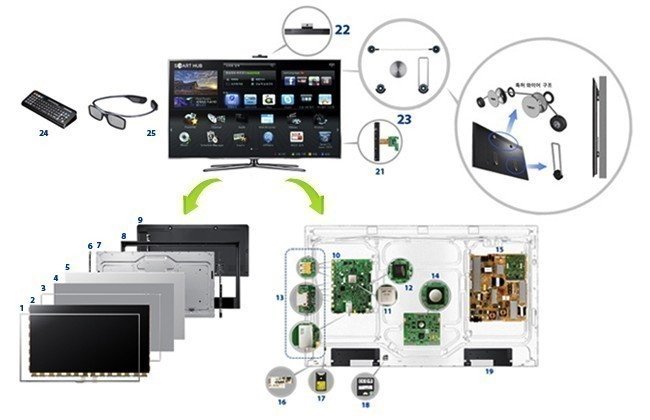
\includegraphics[width=\textwidth]{img/smart_samsung.jpg}
	\caption{\emph{Smart} TV Samsung}
	\label{fig:smart_samsung}
\end{figure}


\subsection{Classificação Indicativa para Conteúdo Televisivo}
%!TEX root = ../sbc-template.tex

O processo de classificação indicativa integra o sistema de garantias dos direitos da criança e do adolescente quanto a promover, defender e garantir o acesso a espetáculos e diversões públicas adequados à condição de seu desenvolvimento, mas reserva-se o direito final aos pais e responsáveis quanto à escolha do conteúdo adequado a estes\cite{eca}.

No Brasil, a \emph{Coordenação de Classificação Indicativa} (Cocind), vinculada ao Ministério da Justiça, é o órgão responsável pela classificação indicativa de obras destinadas à televisão e outros meios, incluindo até mesmo aplicativos. A análise da classificação indicativa realizada pelo Cocind considera o grau de incidência de conteúdos de sexo e nudez, violência e drogas nas obras a serem avaliadas, como sintetizado na Tabela \ref{tab:categorias}. O processo envolve o exame do conteúdo das obras a serem classificadas, a atribuição de classificação indicativa, verificação do cumprimento das normas associadas e advertência por descumprimento destas normas \cite{portaria:ci}.


%!TEX root = ../../novoIndex.tex
\begin{table}[!ht]
  \scalefont{0.8}
  \caption{Categorias de classificação indicativa propostas pela Portaria No. 368, de 11 de Fevereiro de 2014. Fonte: \cite{ci:guia}}
  \label{tab:categorias}
	\centering
	\begin{tabular}{p{4cm} p{1.5cm} p{8cm}}
		\hline
		\textbf{Categoria} & \textbf{Símbolo} & \textbf{Descrição do Conteúdo} \\
		\hline
		Livre & \vfill
\includegraphics[width=0.05\textwidth]{img/livre.png} \vfill&
				Conteúdo predominantemente positivo ou que contem imagens de violência fantasiosa, armas sem violência, mortes sem violência, ossadas e esqueletos sem violência, nudez não erótica e consumo moderado ou inusitado de drogas lícitas. \\
		\hline
		Não recomendado para menores de dez anos &\vfill 
\includegraphics[width=0.05\textwidth]{img/10anos.png}\vfill &
		 		Presença de armas com violência; medo ou tensão; angústia; ossadas e esqueletos com resquícios de ato de violência; atos criminosos sem violência; linguagem depreciativa; conteúdos educativos sobre sexo; descrições verbais do consumo de drogas lícitas; discussão sobre o tráfico de drogas; e o uso medicinal de drogas ilícitas.\\
		\hline
		Não recomendado para menores de doze anos &\vfill 
\includegraphics[width=0.05\textwidth]{img/12anos.png}\vfill &
				Ato violento; lesão corporal; descrição de violência; presença de sangue; sofrimento da vítima; morte natural ou acidental com violência; ato violento contra animais; exposição ao perigo; exposição de pessoas em situações constrangedoras ou degradantes; agressão verbal; obscenidade; \emph{bullying}; exposição de cadáver; assédio sexual; supervalorização de beleza física; supervalorização do consumo; nudez velada; insinuação sexual; carícias sexuais; masturbação não explícita; linguagem chula; linguagem de conteúdo sexual; simulações de sexo; apelo sexual; consumo de drogas lícitas; indução ao uso de drogas lícitas; consumo irregular de medicamentos; menção a drogas ilícitas.\\
		\hline
		Não recomendado para menores de catorze anos &\vfill 
\includegraphics[width=0.05\textwidth]{img/14anos.png}\vfill &
				Morte intencional; estigma ou preconceito; nudez; erotização; vulgaridade; relação sexual não explícita; prostituição; insinuação do consumo de drogas ilícitas; descrições verbais do 	consumo de drogas ilícitas; e discussão sobre a descriminalização de drogas ilícitas.\\
		\hline
		Não recomendado para menores de dezesseis anos &\vfill 
\includegraphics[width=0.05\textwidth]{img/16anos.png}\vfill &
				Estupro; exploração sexual; coação sexual; tortura; mutilação; suicídio; violência gratuita ou banalização da violência aborto, pena de morte ou eutanásia; relação sexual intensa não explícita; produção ou tráfico de qualquer droga ilícita, consumo de drogas ilícitas; indução ao consumo de drogas ilícitas.\\
		\hline
		Não recomendado para menores de dezoito anos &\vfill 
\includegraphics[width=0.05\textwidth]{img/18anos.png}\vfill &
				Violência de forte impacto; elogio, glamourização e/ou apologia à violência; crueldade; crimes de ódio; pedofilia; sexo explícito; situações sexuais complexas ou de forte impacto; apologia ao uso de drogas ilícitas.\\
		\hline
	\end{tabular}
\end{table}


No mundo, conteúdos televisivos são comumente classificados quanto ao grau de incidência de assuntos como linguagem vulgar, conteúdo sexual, drogas e violências, além de temas como conteúdo perturbador e discriminação, a exemplo dos Países Baixos. É frequente a aplicação de restrições de horários para a transmissão de conteúdos restritivos. As classes podem incluir restrição de idade e/ou supervisão de responsáveis, como ocorre nos Estados Unidos, Chile, Equador, Hong Kong, entre outros. Em países como a Austrália e Nova Zelândia, há um sistema de classificação indicativa para televisão aberta e outro para fechada, e um sistema de classificação especial para programas direcionados ao público infantil, na Austrália. Na Colômbia, é proibida a transmissão aérea de pornografia, mesmo em canais adultos. O ícone da classificação indicativa frequentemente deve ser exibido antes do início do programa, antes do início de cada bloco, a exemplo do Brasil, ou durante toda a transmissão do programa, como é o caso da França.  Na Alemanha, apenas o aviso ``O programa a seguir não é recomendado para espectadores abaixo de 16/18 anos'' é mostrado na tela caso haja conteúdo potencialmente ofensivo. Em países como Portugal, Polônia e Singapura, a implantação de sistemas de classificação indicativa é recente, posterior ao ano 2000. \todo{Falta referência}


\subsection{Aprendizagem de Máquina}
Aprendizado de máquina trata de criar modelos que se modificam ou adaptam suas ações para que elas se tornem mais acuradas, enquanto acurácia é medida através do quão bem as ações escolhidas refletem nas corretas.
Um algoritmo que realiza aprendizado de máquina é aquele capaz de aprender a partir de dados, ou experiência, assim como humanos e outros animais. Estes, ao se depararem com determinada, costumam tentar lembrar-se se da última vez em que estiveram em uma situação parecida, tentaram alguma ação que pode ter dado certo -- então deve ser repetida-- ou errado -- então deve tentar algo diferente --adaptação \cite{marsland2015machine}, \cite{goodfellow2016deep}. De acordo com a definição clássica de \cite{mitchell1997machine}, um algoritmo que aprende a partir da experiência $E$ quanto a um conjunto de tarefas $T$ e medida de performance $P$, se sua performance nas tarefas em $T$, medida por $P$, melhora com a experiência $E$.
Algumas tarefas que podem ser atacadas utilizando aprensdizado de máquina são a classificação, regressão, transcrição, tradução automática, detecção de anomalia, síntese e amostragem \cite{goodfellow2016deep}.

\subsection{\emph{Deep Learning}}
Aprendizagem profunda é um conjunto de técnicas de aprendizagem de máquina que se baseiam em modelos com arquiteturas profundas, compostas de vários níveis de operações não lineares, a exemplo das redes neurais com múltiplas camadas escondidas ou um conjunto de fórmulas proposicionais que re-utiliza várias sub-fórmulas \cite{bengio2009learning}. Estes modelos ganharam popularidade com o aumento da quantidade de dados disponíveis sobre temas complexos, aliado com o aumento da disponibilidade de recursos computacionais para executar modelos mais robustos e o aumento de tamanho dos conjuntos de dados disponíveis \cite{goodfellow2016deep}. De acordo com a IBM, são gerados $2,5$ quintilhões de bytes de dados por dia, e $90\%$ do volume de dados presente no mundo hoje foi criado nos últimos dois anos \cite{ibm2017bigdata}.


\subsection{Redes Neurais Convolucionais}
Redes neurais convolucionais (RNC) são um tipo de rede neural específico para o processamento de dados que têm uma topologia bem definida e estruturada em uma grade, a exemplo de séries temporais e imagens. Sua principal característica envolve o uso de convoluções no lugar de multiplicações de matrizes em ao menos uma das camadas da rede neural.\cite{goodfellow2016deep}.

Cada camada das redes neurais convolucionais é composta por uma etapa de convolução, seguida por uma ativação não-linear, finalizando em \emph{pooling}, como mostra a Figura \ref{fig:cnn_camada}. A seguir, serão explanadas cada uma destas etapas.

\begin{figure}
	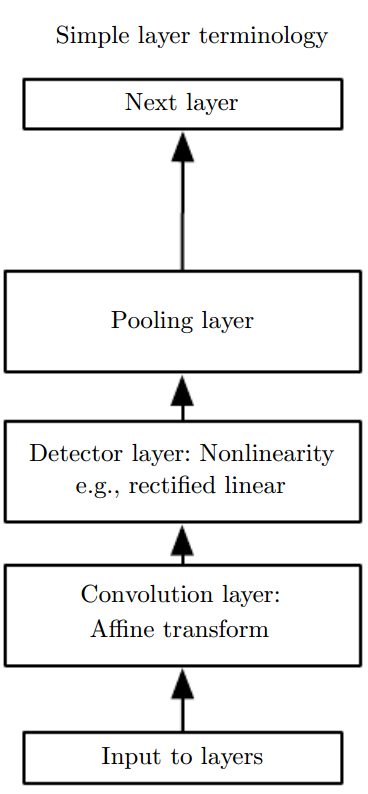
\includegraphics[height=0.5\textheight]{img/cnn_camada.png}
	\caption{Componentes de uma camada de uma rede neural convolucional \cite{goodfellow2016deep}. }
	\label{fig:cnn_camada}
\end{figure}

\subsubsection{Convolução}
A operação de convolução descreve a média ponderada de uma determinada função $x_1(t)$ sob um intervalo fixo de uma variável, enquanto os pesos da média ponderada considerada pertencem à função $x_2(t)$ amostrados em intervalos $a$ \cite{bracewell1986fourier}. Assim, a convolução $s(t)$ de duas funções $x_1(t)$ e $x_2(t)$ é uma função $f: \mathds{Z} \rightarrow \mathds{R}$ representada simbolicamente por $x_1(t) * x_2(t)$ e definida de acordo com a Equação \ref{eq:int_convolucao} \cite{lathi2006sinais}.
\begin{equation}\label{eq:int_convolucao}
	s(t) = x_1(t) * x_2(t) = \int_{-\infty}^{\infty} x_1(a) x_2(t-a)da
\end{equation}

Quando a operação de convolução é aplicada em aprendizagem de máquina, a primeira função $x_1(t)$ é chamada de \emph{input (entrada?)}, a segunda função $x_2(t)$ é chamada de \emph{kernel (núcleo?)}, e a saída $s(t)$ é chamada de mapa de \emph{feature map (mapa de características?)}. Neste caso, a entrada normalmente é um vetor multidimensional de dados e o núcleo é um vetor multidimensional de pesos que devem ser adaptados pelo algoritmo de aprendizado de máquina. Em redes neurais convolucionais, os vetores multidimensionais de entrada e núcleo são chamados tensores. Além disto, assume-se que os valores dos tensores são zero em todos os pontos menos os que estão guardados em memória, ou seja, a operação de convolução é implementada apenas nas posições declaradas dos vetores de dados e peso. Assim, para uma imagem bidimensional de tamanho $(m,n)$ $I$ como entrada, tem-se um núcleo bidimensional $K$, e a operação de convolução é definida como exemplificado na Equação \ref{eq:conv_img}, para cada posição $(i,j)$ do mapa de características resultante \cite{goodfellow2016deep}.

\begin{equation}\label{eq:conv_img}
	S(i,j) = I(i,j)*K(i,j) = \sum_{m}\sum_{n}I(m,n)K(i-m,j-n)
\end{equation}

A convolução é comutativa, ou seja, as Equações \ref{eq:conv_img_eq} e \ref{eq:conv_img} são equivalentes, salvo que no primeiro caso há a convolução da imagem pelo núcleo, enquanto no segundo há a convolução do núcleo pela imagem. Comumente, a Equação \ref{eq:conv_img} é a implementada em algoritmos de redes neurais convolucionais, haja visto que existem menor variação no intervalo de valores válidos de $m$ e $n$, o que diminui o custo computacional.

\begin{equation}\label{eq:conv_img_eq}
	S(i,j) = K(i,j)*I(i,j) = \sum_{m}\sum_{n}I(i-m,j-n)K(m,n)
\end{equation}

A propriedade comutativa surge graças à ação de revolver o núcleo em relação à imagem, e não tem aplicação prática. Porém, esta propriedade não tem fins práticos além da prova da operação de convolução. Assim, é comum que seja implementada correlação cruzada, indicada na Equação \ref{eq:correlacao_img_eq}, semelhante à convolução dada na Equação \ref{eq:conv_img_eq} sem que haja o espelhamento do núcleo em relação à imagem.

\begin{equation}\label{eq:correlacao_img_eq}
	S(i,j) = I(i,j)*K(i,j) = \sum_{m}\sum_{n}I(i+m,j+n)K(m,n)
\end{equation}

\subsubsection{Pooling}

Depois de realizar várias operações de convolução em paralelo para gerar um conjunto de ativações lineares e alimentá-las a funções de ativação não-lineares, como \emph{ReLU}, \emph{Softmax}, etc, na chamada etapa de detecção, chega-se à etapa de \emph{pooling}. Uma função de \emph{pooling} substitui a saída da rede em determinada localização por uma síntese estatística das saídas vizinhas. Por exemplo, a função \emph{max pooling} retorna o valor máximo em uma área retangular, enquanto a \emph{average pooling} retorna a média das saídas de um retângulo. O objetivo destas funções é fazer com que


\subsection{Modelos clássicos de Redes Neurais Convolucionais}
Estes modelos trouxeram grandes inovações quanto à arquitetura das redes neurais convolucionais.
\subsubsection{LeNet}

\subsubsection{AlexNet}

\subsubsection{GoogleLeNet ou Inception}

\subsubsection{ResNet}

\subsubsection{SSD}

\subsubsection{YOLO}

%
% \chapter{Trabalhos Relacionados}\label{sec:trab_relac}
% %!TEX root = ../sbc-template.tex
A proposta apresentada está relacionada com inúmeros trabalhos envolvendo a aplicação de redes neurais convolucionais e outros modelos de \emph{machine learning} para a estimação de idade de indivíduos.

Segundo \cite{fu2010age}, a idade pode ser inferida a partir de padroões distintos que emergem através da aparência da face. Técnicas comuns para a estimação da idade envolvem a dedução de modelos matemáticos a partir do estudo do crescimento de medidas da face e do crânio \cite{kwon1999age}, da textura do rosto \cite{lanitis2002toward}, da captura de tendências de envelhecimento a partir de várias imagens de indivíduos de mesma idade \cite{fu2007estimating} e a extração de características específicas relacionadas à idade \cite{suo2008design}, \cite{lou2018expression}. Modelos de \emph{machine learning} também são utilizados para a tarefa, em especial as redes neurais artificiais, K-vizinhos mais próximos e máquinas de vetores de suporte.

Recentemente, a aplicação de redes neurais convolucionais em problemas de classificação e detecção de objetos em imagens têm obtido resultados significativamente positivos. Em \cite{vggnet}, \cite{resnet}, \cite{inception}, \cite{redmon2016you}, \cite{ssd} e outros, são descritas arquiteturas robustas capazes de detectar dezenas de objetos em várias situações. Treinadas com conjuntos de dados visuais que contam com milhares de exemplos como a ImageNet, Pascal VOC e COCO, estas redes são conhecidas por seu bom desempelho. Algumas destas redes foram afinadas utilizando conjuntos de dados menores e especializados para a tarefa de estimação de idade.

O trabalho de \cite{rothe2015dex} relata um método para estimação de idade aparente em imagens de faces imóveis utilizando \emph{deep learning}. Propõe-se um conjunto de $20$ redes neurais convolucionais classificadoras com arquiteturas VGG-16 pré-treinadas com a base de dados visuais ImageNet, e ajustadas utilizando imagens disponibilizadas pelo IMDB, Wikipedia, e o conjunto de dados \emph{Looking At People}--LAP para anotação de idade aparente. Cada modelo tem como saída um número discreto entre $0$ e $100$, representando a idade prevista. A saída final do modelo consiste na média entre as idades previstas pelos $20$ redes. A solução atingiu um MAE (\emph{Mean Average Error}) de $3.221$ na fase de testes.

Em \cite{liu2015agenet} cria-se um estimador de idade composto pela fusão de um modelo regressor e outro classificador. Realiza-se um pré-processamento da entrada, que envolve a detecção das faces presentes na imagem, seguida pela etapa de localização de pontos de referência, como olhos, nariz e boca, e por fim há a normalização da face. Dois métodos de normalização de face são testados, a normalização exterior e interior. Após este pré-processamento, as imagens resultantes são alimentadas a modelos de redes neurais convolucionais profundas inspiradas na \emph{GoogLeNet} \cite{inception}. O modelo sofreu modificações em sua arquitetura, como adição de normalização do batch, remoção de camadas de \emph{dropout} e perda. Foram treinados e testados diversos modelos com variações no tipo de normalização da face, tamanho do corte dos rostos, tipo de tarefa preditiva, etc. Os modelos resultantes destas variações foram unidos em um conjunto, que conseguiu prever idades com MAE de $3.3345$.

Ademais, é possível encontrar resultados satisfatórios para a tarefa de aprendizado proposta utilizando modelos menos complexos. Com o objetivo de consolidar um método de classificação de idade e gênero, \cite{levi2015age} propõe uma rede neural convolucional de natureza mais simples, se comparada com \cite{inception}, \cite{vggnet} ou \cite{resnet}. Sua arquitetura consiste em três camadas convolucionais com \emph{dropout} e funções de ativação \emph{ReLU}, seguidas por três camadas totalmente conectadas. A camada de saída tem como função de ativação a Softmax. A escolha por um design de rede menor é motivado pelo desejo de reduzir o risco de \emph{overfitting} e pela natureza do problema, que contém apenas 8 classes de idade. O modelo é treinado utilizando apenas o conjunto de referência \emph{Adience}, composto por imagens não filtradas para classificação de idade e gênero. Considerando uma margem de erro de uma classe vizinha, a melhor rede obteve acurácia de $84.7\% \pm 2.2$ ao empregar a técnica de sobre-amostragem.


\chapter{Solução Proposta}\label{sec:solucao_proposta}
%!TEX root = ../novoIndex.tex
A solução proposta para a realização deste trabalho compreende a especificaçao de técnicnas de DL empregadas para a tarefa de aprendizado tratada. A caracterização da tarefa de aprendizado está exposta na Seção \ref{subsec:tarefa}. A descrição do conjunto de dados está na Seção \ref{subsec:dataset}. A Seção \ref{subsec:limpeza} compreende a limpeza, o pré-processamento e a consolidação do conjunto de dados. Por fim, na Seção \ref{subsec:modelos} estão os modelos, parâmetros e hiperparâmetros de CNNs considerados.

\section{Tarefa de Aprendizado}\label{subsec:tarefa}
%!TEX root = ../../novoIndex.tex
A tarefa de aprendizado considerada para a estimação de idade de telespectadores é a regressão. Neste contexto, uma imagem em cores RGB de dimensões $224 \times 224$ pixels contendo uma face humana centralizada será fornecida como entrada. A saída desejada é a estimativa de idade, em anos, da pessoa correspondente, conforme exemplificado na Figura \ref{fig:deniro_cnn}. Esta tarefa será abordada segundo o paradigma de aprendizado supervisionado.

\begin{figure}[!ht]
  \centering
     \caption{Tarefa de aprendizado}
     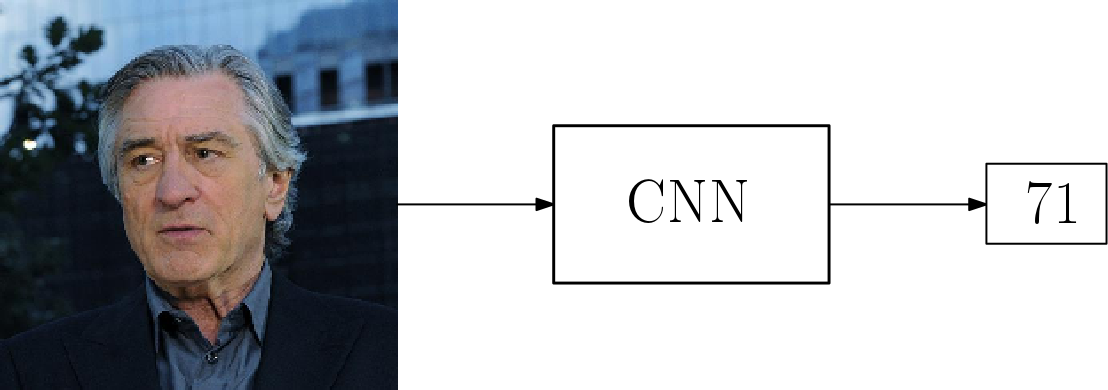
\includegraphics[width=0.8\textwidth]{img/deniro_cnn}
     \label{fig:deniro_cnn}
\end{figure}

Os dados disponíveis para este contexto serão particionados em três conjuntos disjuntos, sendo $70\%$ reservados para o treino, $10\%$ para validação e $20\%$ para teste. Esta partição obedece à tecnica \emph{Holdout} de validação cruzada \cite{brink2016real}.

Os modelos propostos para esta tarefa terão seu desempenho aferido perante os dados do conjunto de testes de acordo com a métrica de desempenho \emph{Root Mean Squared Error} (RMSE). Esta métrica considera a diferença entre cada um dos valores previstos $\hat{y}$ e os reais $y$, e posteriormente quantifica uma média imune à variação positiva ou negativa desta diferença. A Equação \ref{eq:rmse} denota o cálculo do RMSE \cite{brink2016real}.

\begin{equation}\label{eq:rmse}
     \textrm{RMSE} = \sqrt{\frac{1}{n} \sum_{i=1}^n (y_i - \hat{y})^2}.
\end{equation}


\section{Conjunto de Dados}\label{subsec:dataset}
%!TEX root = ../sbc-template.tex
Para a tarefa de aprendizado apresentada, dispôs-se da base de dados experimentais IMDb, composta de $452.132$ exemplares contendo imagens e outras informações de $20.284$ dos atores mais populares listados no site IMDb. O conjunto de dados foi construído utilizando técnicas de \emph{web crawling} aplicadas aos perfis de atores do site, em que foram coletadas todas as imagens relacionadas à celebridade, além de informações como data de nascimento, nome e gênero \cite{IMDb_derivada}.

A base de imagens oriunda do site IMDb foi organizada por Rothe et al. considerando uma tarefa de aprendizado análoga à deste trabalho, conforme mencionado na Seção  \ref{sec:trab_relac} \cite{rothe2015dex}.  Nesta base, há também as coordenadas da localização de um rosto detectado na imagem, além de uma pontuação atribuída ao rosto produzida pelo detector de face, quantificando o grau de certeza na detecção do rosto. Partindo da possibilidade de haver mais de um rosto por imagem, uma segunda pontuação é atribuída pelo detector, referente ao grau de certeza de que há outro rosto na mesma imagem.

Neste contexto, cada exemplo deste conjunto de dados é referente a uma imagem, cujos meta-dados estão descritos em seus atributos, que compreendem o nome, gênero, data de nascimento e um número de identificação da celebridade cujo perfil estava atrelado à imagem, o endereço da foto em disco, a suposta localização da face da celebridade, e pontuações referentes a duas possíveis faces encontradas. Assim, há exemplos de imagens em que há apenas um rosto, como mostrado na Figura \ref{tab:um_deniro}. Já na Figura \ref{tab:dois_deniro_correto} está o exemplo de uma imagem onde há mais de um rosto, porém a localização do rosto está correta. Por fim, na Figura \ref{tab:dois_deniro_errado} há uma imagem com mais de um rosto, porém o rosto identificado neste item não é o da celebridade cujos dados estão referenciados.

\begin{figure}[ht]
     \caption{Exemplo de imagem do conjunto de dados contendo apenas um rosto.}
     \label{tab:um_deniro}
          \begin{minipage}[c]{0.62\linewidth}
          \begin{small}
          \centering
          \begin{tabular}{p{3.3cm} p{5cm}}\toprule
               \textbf{Meta-dado} & \textbf{Valor} \\ \midrule
               ID Celebridade & 16349 \\
               Nome & Robert De Niro \\
               Endereço da imagem & \footnotesize{imdb$/$34$/$nm0000134$\_$rm334009 0368$\_$1943-8-17$\_$2011.jpg} \\
               Pontuação da Face & $5.21396$ \\
               Pontuação da Segunda Face & NaN \\
               Localização da Face & $(663.65, 992.475, $ $590.134, 918.959)$ \\
               Data de Nascimento  & $1943-08-17$\\
               Ano da Foto & 2011 \\
               Gênero & Masculino \\
               \bottomrule
          \end{tabular}
     \end{small}
     \end{minipage}
     \hfill
     \begin{minipage}[c]{0.35\linewidth}
          \centering
          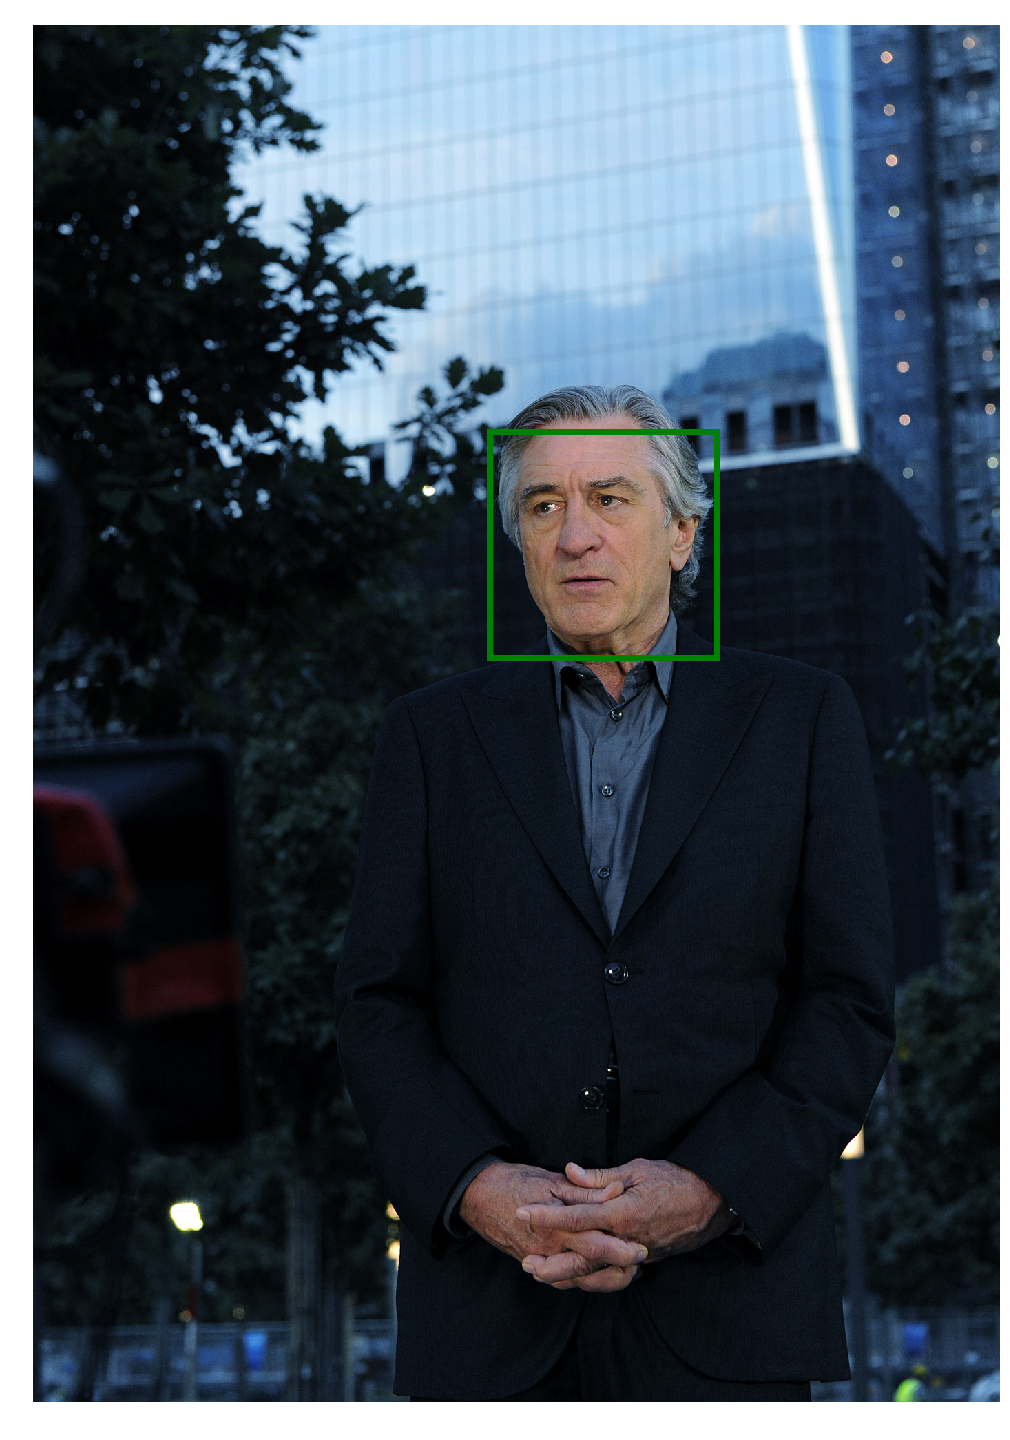
\includegraphics[width=\linewidth]{img/deniro_plt}
     \end{minipage}
\end{figure}

\begin{figure}[ht]
     \caption{Exemplo de imagem do conjunto de dados contendo mais de um rosto com a classificação correta.}
     \label{tab:dois_deniro_correto}
          \begin{minipage}[c]{0.62\linewidth}
          \begin{small}
          \centering
          \begin{tabular}{p{3.3cm} p{5cm}}\toprule
			   \textbf{Meta-dado} & \textbf{Valor} \\ \midrule
               ID Celebridade & 16349 \\
               Nome & Robert De Niro \\
               Endereço da imagem & \footnotesize{imdb$/$34$/$nm0000134$\_$rm17663 60064$\_$1943-8-17$\_$2010.jpg} \\
               Pontuação da Face & $5.12527$ \\
               Pontuação da Segunda Face & $5.08887$ \\
               Localização da Face & $(914.886, 1426.31, $ $287.31, 798.734)$ \\
               Data de Nascimento  & $1943-08-17$\\
               Ano da Foto & 2010 \\
               Gênero & Masculino \\
               \bottomrule
          \end{tabular}
     \end{small}
     \end{minipage}
     \hfill
     \begin{minipage}[c]{0.35\linewidth}
          \centering
          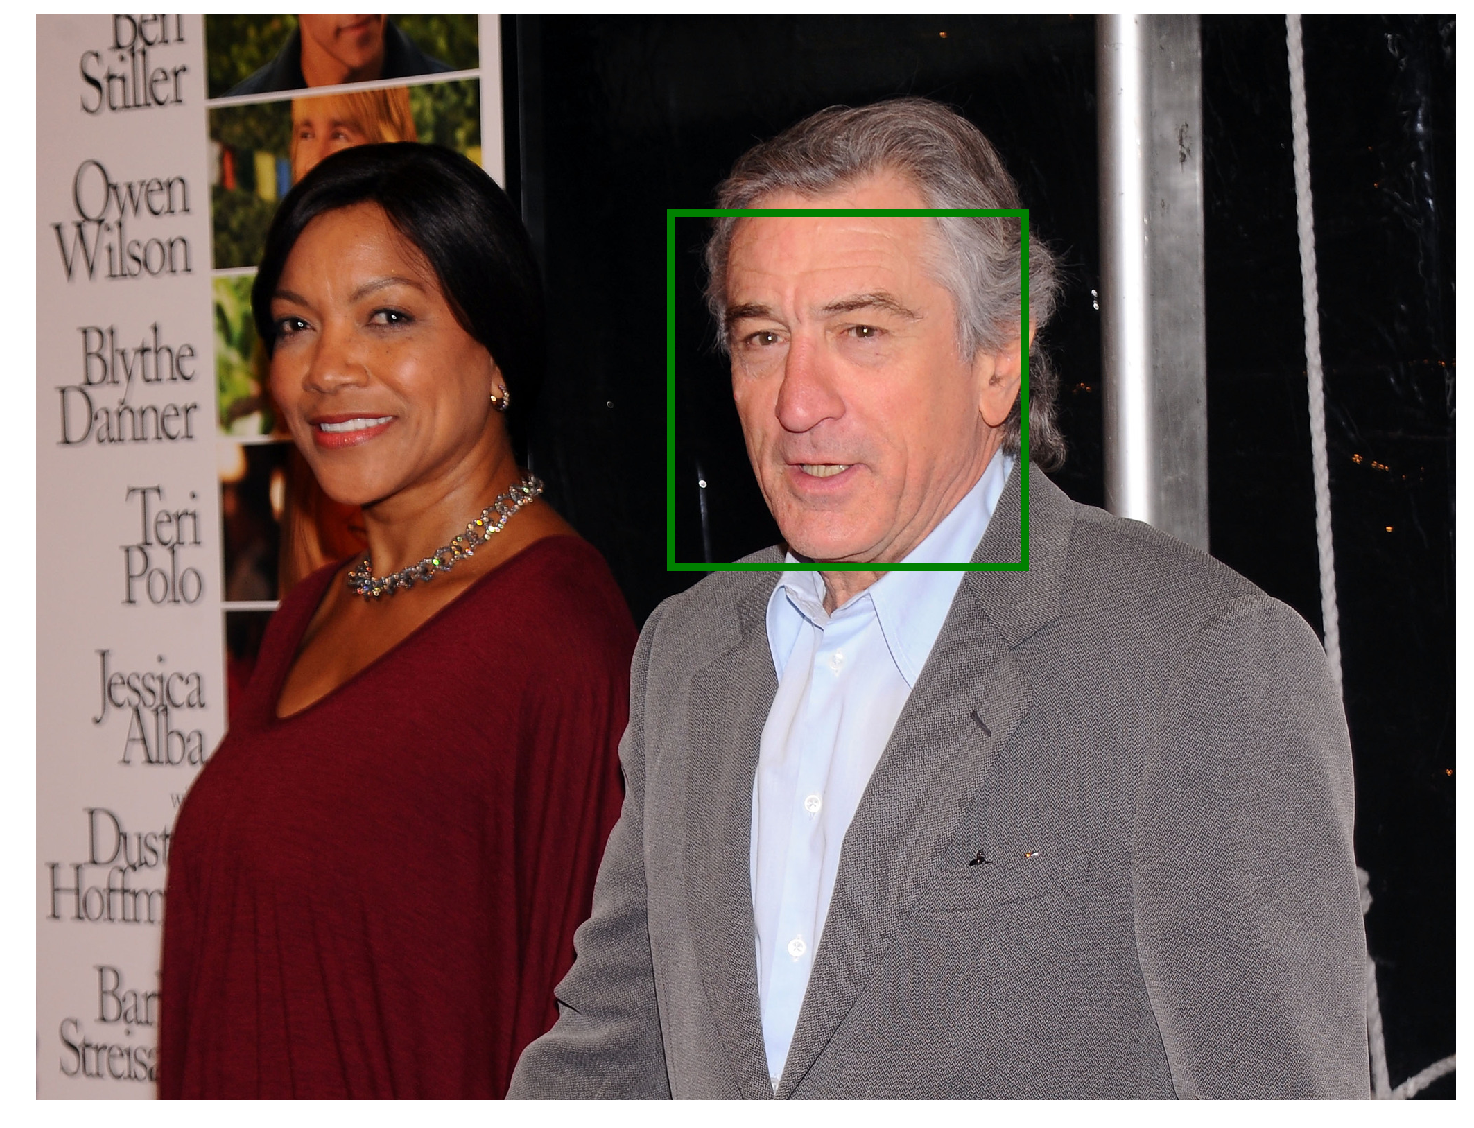
\includegraphics[width=\linewidth]{img/deniro_many_plt_correto}
     \end{minipage}
\end{figure}

\begin{figure}[ht]
     \caption{Exemplo de imagem do conjunto de dados contendo mais de um rosto com a classificação errônea.}
     \label{tab:dois_deniro_errado}
          \begin{minipage}[c]{0.62\linewidth}
          \begin{small}
          \centering
          \begin{tabular}{p{3.3cm} p{5cm}}\toprule
               \textbf{Meta-dado} & \textbf{Valor} \\ \midrule
               ID Celebridade & 16349 \\
               Nome & Robert De Niro \\
               Endereço da imagem & \footnotesize{imdb$/$34$/$nm0000134$\_$rm14800 44288$\_$1943-8-17$\_$2012.jpg} \\
               Pontuação da Face & $5.51656$ \\
               Pontuação da Segunda Face & $4.55379$ \\
               Localização da Face & $(1392.72, 1614.18, $ $225.55, 447.003)$ \\
               Data de Nascimento  & $1943-08-17$\\
               Ano da Foto & 2012 \\
               Gênero & Masculino \\ \bottomrule
          \end{tabular}
     \end{small}
     \end{minipage}
     \hfill
     \begin{minipage}[c]{0.35\linewidth}
          \centering
          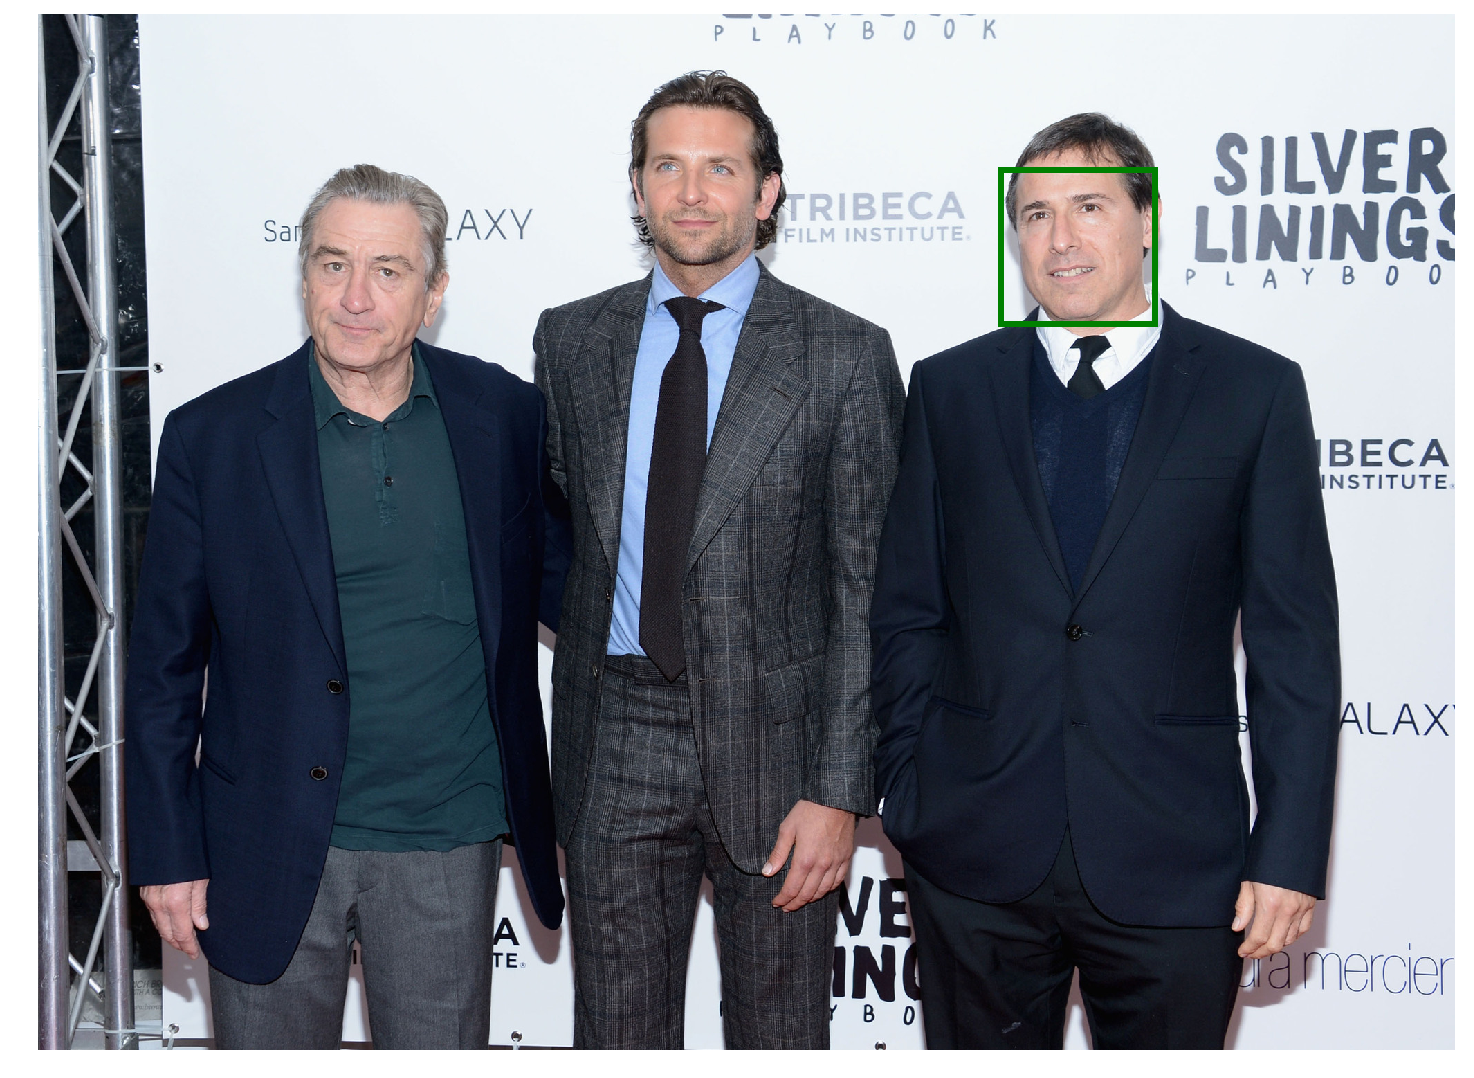
\includegraphics[width=\linewidth]{img/deniro_many_plt_errado}
     \end{minipage}
\end{figure}

A versão original das imagens do conjunto de dados IMDb ocupava 267 GB em disco. Porém, uma versão pré-processada dessas imagens está disponível, contendo as faces recortadas com $40\%$ da largura e altura da imagem original, totalizando $7,1$ GB de dados. Esta versão foi considerada neste trabalho.


\section{Limpeza e Pré-processamento dos dados}\label{subsec:limpeza}
%!TEX root = ../../novoIndex.tex
A fim de adequar melhor o conjunto de dados para os modelos de CNNs utilizados, realizou-se uma limpeza e pré-processamento dos meta-dados e das imagens da base IMDb, que se iniciou com o cálculo do atributo alvo, a idade, a partir dos atributos originais fornecidos. A idade foi aferida através da data de nascimento da celebridade e do ano em que a fotografia em questão foi capturada.

Uma análise do conjunto de dados revelou a presença de itens com idade e gênero apresentando valores nulos, inválidos ou negativos, que foram descartados. Observou-se também a presença de múltiplos exemplos referentes à mesma pessoa com a mesma idade. Houve a remoção de tais exemplos, a fim de evitar que a apresentação de um mesmo rosto com a mesma idade provocasse \emph{overfitting} nos modelos. Exemplos atípicos, possivelmente resultados de rotulação incorreta, como idade maior que $100$ anos ou não compatível com os dados da celebridade referida nos meta-dados também foram descartados. Os atributos de pontuação de rostos foram úteis para identificar e remover exemplos em que não havia nenhum rosto identificado, ou em que havia mais de uma face na imagem. Este descarte foi realizado com o objetivo de eliminar rotulações errôneas, como a mostrada na Tabela \ref{tab:dois_deniro_errado}.

Foram realizados também procedimentos de pré-processamento nas imagens. Considerando a literatura, padronizou-se o modo RGB e o tamanho das imagens para $224 \times 224$ \emph{pixels}. A seguir, realizou-se a equalização do histograma de cores das imagens, a fim de aumentar o contraste global e evidenciar características das faces, como mostrado na Figura \ref{fig:equalizacao} \cite{}. A normalização realizada a seguir teve como objetivo manter os valores de entrada entre 0 e 1, dividindo os pixeis das imagens por $255$. Este último processo evita que as RNAs prevejam a média dos valores de entrada.

\begin{figure}[!ht]
	\caption{Exemplo de imagem do conjunto de dados antes e depois do processo de equalização por histograma.}
	\label{fig:equalizacao}
	\centering
	\begin{subfigure}[h]{0.4\linewidth}
		\caption{Imagem sem normalização por equalização de histograma.}
		\label{fig:slp}
		\centering
		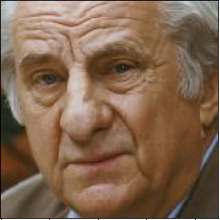
\includegraphics[width=0.8\linewidth]{img/solucao/hist_eq_orig.png}
	\end{subfigure}
	\hspace{0.1cm}
	\begin{subfigure}[h]{0.4\linewidth}
		\caption{Imagem após normalização por equalização por histograma.}
		\label{fig:rbm}
		\centering
		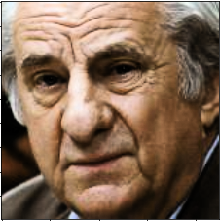
\includegraphics[width=0.8\linewidth]{img/solucao/hist_eq_mod.png}
	\end{subfigure}
\end{figure}

Após o pré-processamento das imagens de entrada, o cálculo do atributo alvo idade, a adequação do caminho para as imagens em disco e a remoção de exemplos impróprios, seguiu-se o descarte dos outros meta-dados irrelevantes para a tarefa de estimação de idade de um indivíduo a partir de imagem. A data em que a foto foi tirada, nome, número de identificação, gênero, data de nascimento, localização do rosto da celebridade e pontuações de rostos nas imagens foram removidos.

\begin{figure}[!ht]
    \centering
     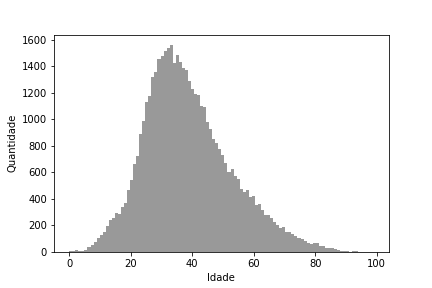
\includegraphics[width=0.7\textwidth]{img/idade_hist_clean}
     \caption{Histograma de frequência da idade do conjunto de dados utilizado.}
     \label{fig:hist}
\end{figure}

Por fim, o conjunto de dados consolidado consiste de $47.950$ exemplos contendo imagens e idades de $14.607$ celebridades distintas, ocupando $1,2 GB$. O histograma de frequência da distribuição de idades de 0 a 100 anos presente nos exemplos da base de dados pode ser visualizado na Figura \ref{fig:hist} \cite{acharya2005image}. Este total foi então dividido como proposto: conjunto de treinamento, contendo $70\%$ dos exemplos, ou seja, $33.565$ amostras; conjunto de validação, referente a $10\%$ dos dados, ou seja, $4.795$ itens; e, por fim, conjunto de testes, contendo os $20\%$ restantes, ou seja, $9.590$ exemplos.


\section{Modelos de CNN Considerados} \label{subsec:modelos}
%!TEX root = ../../novoIndex.tex
Levando em conta a adoção de CNNs como o modelo de ML a ser usado neste trabalho, considerou-se a utilização das arquiteturas LeNet e AlexNet. A implementação da AlexNet seguiu a prática atual de utilizar apenas uma GPU em seu treinamento, então as camadas dividas no trabalho original foram unificadas \cite{tensorflow:alexnet}. Todas as funções de ativação tangente hiperbólica disponíveis nas versões originais destas redes foram substituídas pela função \emph{ReLU}, por ser mais eficiente computacionalmente, evitar que o gradiente descendente tenda a zero e por promover uma convergência mais rápida \cite{maas2013rectifier}. Adotou-se um \emph{batch size} igual a $64$ para o treinamento, e o método de otimização do gradiente descendente foi o \emph{Adam}. O número de épocas e a taxa de aprendizado foram obtidas de maneira experimental, observando a perda obtida ao final de cada época.

A fim de caracterizar a tarefa de regressão proposta, as camadas de saída da LeNet e AlexNet com múltiplos neurônios voltados à classificação foram substituídas por apenas um neurônio com função de ativação \emph{ReLU}. Após análise dos resultados preliminares obtidos para estes modelos iniciais, substituiu-se a \emph{ReLU} da camada de saída por uma de suas variantes, chamada \emph{Leaky ReLU}, e expressa na Figura \ref{fig:lrelu}. A taxa de aprendizado inicial foi padronizada em um valor de $10^{-3}$ com decaimento de $10^{-10}$ para ambas as redes.

\begin{figure}[!ht]
     \centering
     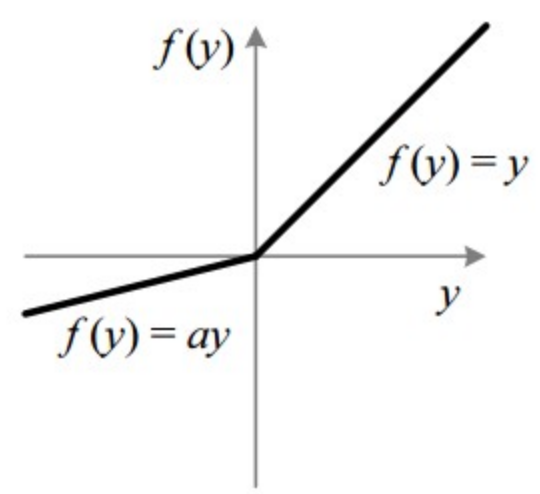
\includegraphics[width=0.3\textwidth]{img/lrelu}
     \caption{Função de Ativação \emph{Leaky ReLU}}
     \label{fig:lrelu}
\end{figure}

Na seção a seguir estão os resultados preliminares obtidos do treino dos modelos, hiperparâmetros e estratégias supracitados.



\chapter{Resultados e Discussão}
%!TEX root = ../novoIndex.tex

Considerando a abordagem descrita na solução proposta, os resultados da execução das CNNs aplicadas ao problema de estimação de idade a partir de uma imagem de face são apresentados a seguir.

%
\subsection{Abordagem do TCC1}

A primeira abordagem de treinamento das CNNs constitiu na utilização das imagens da base de dados sem pré-processamento. Conforme mencionado na Seção \ref{subsec:modelos}, os primeiros treinamentos e testes compreenderam as arquiteturas canônicas LeNet e AlexNet com função de ativação \emph{ReLU} na camada de saída, tendo como entrada as imagens do conjunto de dados sem normalização e equalização. Obedecendo ao método de validação cruzada \emph{holdout} previamente mencionado, os resultados da etapa de teste foram obtidos, detalhados na Tabela \ref{tab:results_relu}.

\begin{table}[!ht]
     \caption{Resultados preliminares do treino e teste dos modelos propostos utilizando \emph{ReLU} na camada de saída.}
     \label{tab:results_relu}
     \centering
     \begin{tabular}{l l l}
          \toprule
          Modelo & Épocas &RMSE \\
          \midrule
          LeNet & $95$ & $41.08$ \\
          AlexNet & $55$ & $41.96$\\
          \bottomrule
     \end{tabular}
\end{table}

Ao observar as previsões realizadas para exemplos individuais, percebeu-se uma tendência destas redes após treinamento em preverem valores baixos, indicando possivelmente \emph{underfitting} em virtude do \emph{ReLU dying problem} \cite{djork2015elus, dabal2018elus}. Como alternativa, estes autores sugerem  utilizar variantes da \emph{ReLU} que não exibam saídas nulas, diferentes estratégias de inicialização e regularização de pesos e \emph{batches}, entre outras. Como exposto na Seção \ref{subsec:modelos}, adotou-se a \emph{Leaky ReLU} como função de ativação da camada de saída. Os resultados deste treinamento estão expostos na Tabela \ref{tab:results_leaky}.

\begin{table}[!ht]
     \caption{Resultados preliminares do treino e teste dos modelos propostos utilizando \emph{Leaky ReLU} na camada de saída.}
     \label{tab:results_leaky}
     \centering
     \begin{tabular}{l l l}
          \toprule
          Modelo & Épocas & RMSE \\
          \midrule
          LeNet & $12$ & $41.55$ \\
          AlexNet & $6$ & $14.38$\\
          \bottomrule
     \end{tabular}
\end{table}

Observa-se que houve uma resposta positiva da AlexNet que melhorou a qualidade das previsões para o problema considerado. Porém, observa-se uma tendência desta rede em prever valores médios, o que ainda enseja melhorias. Assim, ainda é necessário investigar outros parâmetros e modelos para o problema em questão.


\subsection{Abordagem 1}%fase2
A primeira abordagem de treinamento das CNNs utilizou as imagens da base de dados com equalização por histograma de frequência, normalizadas, e com $50\%$ de chance de estarem rotacionadas horizontalmente. Conforme mencionado na Seção \ref{subsec:modelos}, os treinamentos e testes compreenderam as arquiteturas canônicas LeNet e AlexNet com funções de ativação \emph{ReLU} e \emph{Leaky ReLU} nas camadas ocultas e de ativação. É importante ressaltar que neste momento não foram utilizadas técnicas de \emph{transfer learning}.

% Explicação da le net, gráficos da le net
A CNN que implementa a arquitetura LeNet com função de ativação \emph{ReLU} foi treinada por 43 épocas, obteve MAE de $14.09$ e RMSE $17.93$. A LeNet com função de ativação \emph{Leaky ReLU} foi treinada por 15 épocas, obteve MAE de $14.44$ anos e RMSE de $18.18$ anos. Os treinamentos duraram aproximadamente $16$ e $12$ horas respectivamente, em uma instância do Google Compute Engine com 4 CPus virtuais e 15 GB de RAM. Os gráficos de treinamento e as retas zero obtidas a partir da apresentação do conjunto de teste aos modelos consolidados podem ser vistos na Figura \ref{fig:lenet-abordagem1}. É possível notar que ambas as redes sofreram com overfitting e obtiveram grande margem de erro, no entanto a LeNet que utilizou \emph{Leaky ReLU} como função de ativação obteve um desempenho mais satisfatório.
.
\begin{figure}[hb!]
	\caption{Resultados do treinamento e teste da CNN LeNet.}\label{fig:lenet-abordagem1}
  \begin{subfigure}[hb]{0.5\linewidth}
    \caption{RMSE de treinamento da arquitetura LeNet utilizando funções de ativação \emph{ReLU}.}
    \label{fig:redeneuralbiologica}
    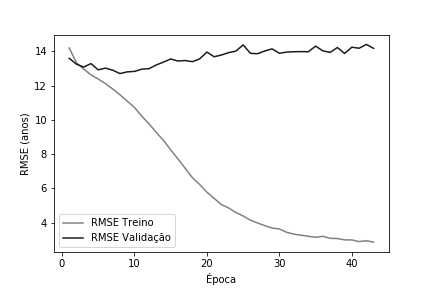
\includegraphics[width=\linewidth]{img/graficos-fase2/fig-history-lenet-relu-data-augmentation-2-1.png}%
  \end{subfigure}%
	\begin{subfigure}[hb]{0.5\linewidth}
		\caption{Reta-0 LeNet \emph{ReLU}.}
		\label{fig:redeneuralbiologica}
		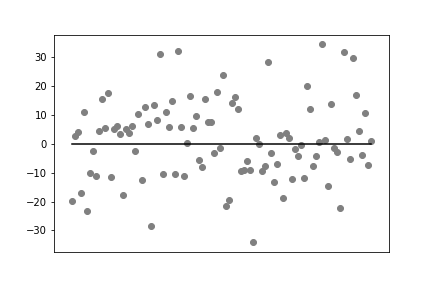
\includegraphics[width=\linewidth]{img/graficos-fase2/fig-reta-0-lenetregressor-relu-data-augmentation-2-1.png}%
	\end{subfigure}\\
  \begin{subfigure}[hb]{0.5\linewidth}
    \caption{RMSE de treinamento da arquitetura LeNet utilizando funções de ativação \emph{Leaky ReLU}.}
    \label{fig:redeneuralbiologica}
    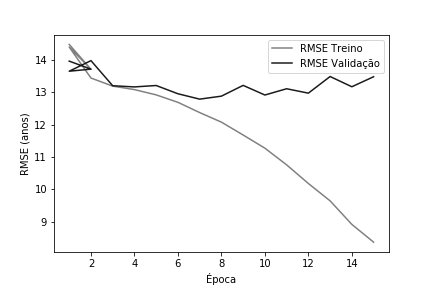
\includegraphics[width=\linewidth]{img/graficos-fase2/fig-history-lenet-lrelu-data-augmentation-2-2.png}
  \end{subfigure}
	\begin{subfigure}[hb]{0.5\linewidth}
		\caption{Reta-0 LeNet \emph{Leaky ReLU}.}
		\label{fig:redeneuralbiologica}
	 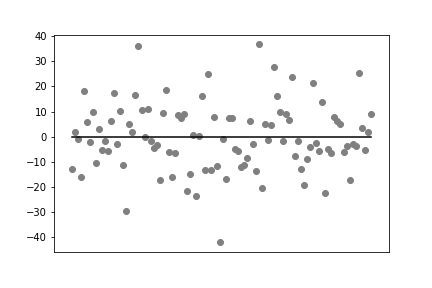
\includegraphics[width=\linewidth]{img/graficos-fase2/fig-reta-0-lenetregressor-lrelu-data-augmentation-2-2.png}
	\end{subfigure}%
\end{figure}

A CNN que implementa a arquitetura AlexNet com função de ativação \emph{ReLU} foi treinada por 10 épocas, obteve MAE de $38.63$ anos e RMSE de $41.22$ anos. A AlexNet com função de ativação \emph{Leaky ReLU} foi treinada por 30 épocas, obteve MAE de $14.44$ anos e RMSE de $15.33$ anos. Os treinamentos duraram aproximadamente $15$ e $38$ horas respectivamente, na mesma instância do Google Compute Engine utilizada para o treinamento das redes LeNet. Os gráficos de treinamento e as retas zero obtidas a partir da apresentação do conjunto de teste aos modelos consolidados podem ser vistos na Figura \ref{fig:alexnet-abordagem1}. É possível notar que a AlexNet que utiliza \emph{ReLU} sofreu de \emph{dying ReLU problem}, o que culminou em previsões iguais a zero para todos os exemplos do conjunto de teste, o que pode ser evidenciado pela ausência total de acertos conforme mostra a Figura \ref{fig:reta0reludying}. Para contornar este problema, a AlexNet que utilizou \emph{Leaky ReLU} como função de ativação foi capaz de convergir para uma solução mais adequada, prevendo idades mais próximas às reais.

\begin{figure}[hb!]
	\caption{Resultados do treinamento e teste da CNN AlexNet.}\label{fig:alexnet-abordagem1}
	\begin{subfigure}[hb]{0.5\linewidth}
		\caption{Treinamento AlexNet \emph{ReLU}.}
		\label{fig:redeneuralbiologica}
		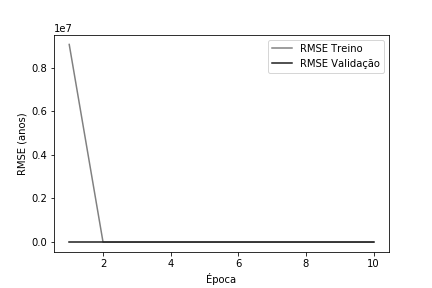
\includegraphics[width=\linewidth]{img/graficos-fase2/fig-history-alexnet-relu-data-augmentation-2-1.png}
	\end{subfigure}
  \begin{subfigure}[hb]{0.5\linewidth}
    \caption{Reta-0 AlexNet \emph{ReLU}.}
    \label{fig:reta0reludying}
    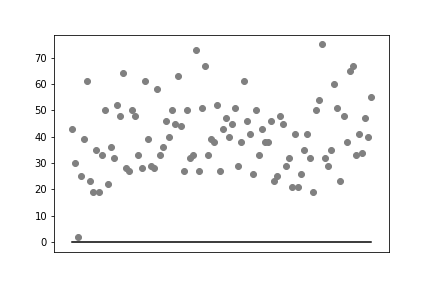
\includegraphics[width=\linewidth]{img/graficos-fase2/fig-reta-0-alexnet-relu-data-augmentation-2-1.png}%
  \end{subfigure}\\
	\begin{subfigure}[hb]{0.5\linewidth}
		\caption{Treinamento AlexNet \emph{Leaky ReLU}.}
		\label{fig:histalexlrelunorm}
    \centering
		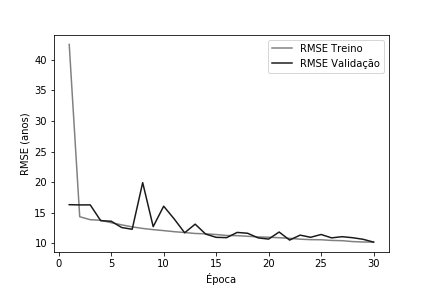
\includegraphics[width=\linewidth]{img/graficos-fase2/fig-history-alexnet-lrelu-data-augmentation-2-2.png}
	\end{subfigure}
  \begin{subfigure}[hb]{0.5\linewidth}
    \caption{Reta-0 AlexNet \emph{Leaky ReLU}.}
    \label{fig:redeneuralbiologica}
    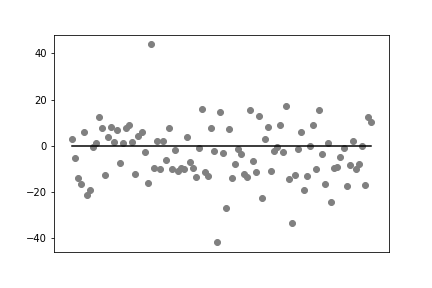
\includegraphics[width=\linewidth]{img/graficos-fase2/fig-reta-0-alexnet-lrelu-data-augmentation-2-2.png}
  \end{subfigure}%
\end{figure}


\begin{figure}[hb!]
	\caption{Redes neurais biológicas.}
	\begin{subfigure}[hb]{0.5\linewidth}
		\caption{Reta-0 Alexnet LRelU com imagens normalizadas e equalizadas}
		\label{fig:histalexlrelunorm}
		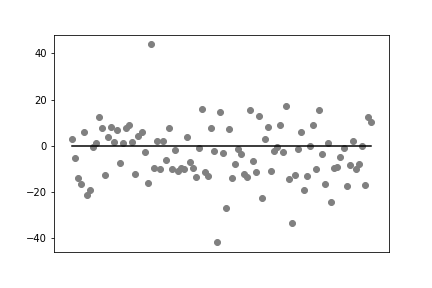
\includegraphics[width=\linewidth]{img/graficos-fase2/fig-reta-0-alexnet-lrelu-data-augmentation-2-2.png}
	\end{subfigure}%
	\begin{subfigure}[hb]{0.5\linewidth}
		\caption{Reta-0 Alexnet ReLU com imagens normalizadas e equalizadas}
		\label{fig:redeneuralbiologica}
		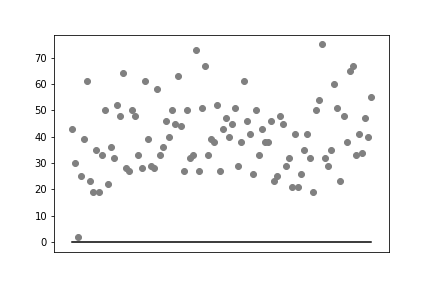
\includegraphics[width=\linewidth]{img/graficos-fase2/fig-reta-0-alexnet-relu-data-augmentation-2-1.png}
	\end{subfigure}
\end{figure}

Obedecendo ao método de validação cruzada \emph{holdout} previamente mencionado, os resultados desta abordagem encontram-se sintetizados na Tabela \ref{tab:results-2}.

\begin{table}[!ht]
	\caption{Resultados do treino e teste dos modelos propostos na Abordagem 1.}
	\label{tab:results-2}
	\begin{adjustbox}{width=1\textwidth}
		\begin{tabular}{l l l l l l l}
			\toprule
			Rede & Função de ativação & Parâmetros & Épocas & Tempo de treinamento & MAE Teste & RMSE Teste \\
			\midrule
			LeNet & \emph{Leaky ReLU} & params & 15 & 12 h & 14.44 & 18.18 \\
			LeNet & \emph{ReLU} & params & 43 & 16 h & 14.09 & 17.93 \\
			AlexNet & \emph{ReLU} & $58.286.145$ & 10 & 15 h & 38.63 & 41.22 \\
			AlexNet & \emph{Leaky ReLU} & params & 30 & 40 h & 15.33 & 18.58 \\
			\bottomrule
		\end{tabular}
	\end{adjustbox}
\end{table}

\subsection{Abordagem 2}

- Mesmas redes
- Normalização das imagens, equalização por histograma -> o que é
- data augmentation ->  mais técnicas de data augmentation

\subsection{Abordagem 3}

Outras arquiteturas
VGG
com transfer learning
1. Retirar última camada (softmax) e adicionar leaky relu
2. Retirar duas últimas camadas (dense e softmax) e adicionar leaky relu
\label{sec:resultados}

\chapter{Considerações Finais}\label{sec:consid_finais}
%!TEX root = ../sbc-template.tex
O objetivo deste trabalho consiste em elaborar estratégias inteligentes para estimação de idade de telespectadores de  \emph{Smart} TVs a partir de suas respectivas fotografias faciais. Para este fim, foram propostos, treinados e testados em caráter preliminar dois modelos de CNNs já bem estabelecidos na literatura, a LeNet e AlexNet, com dois perfis de hiperparâmetros cada um.

Ao observar as previsões realizadas pelas primeiras configurações de LeNet e AlexNet propostas, notou-se que ambas exibiam saídas iguais a zero para quaisquer imagens de entrada. Concluiu-se que as redes estavam sofrendo do chamado \emph{ReLU dying problem}, ou problema da morte da \emph{ReLU}. Considerando o gráfico desta função de ativação exibido na Tabela \ref{tab:ativacoes}, nota-se que a \emph{ReLU} exibe saída $0$ para entradas com valores negativos, e saída linear para entradas positivas.
%Sua derivada, também exibida na Tabela \ref{tab:ativações}, é igual a zero para valores negativos e 1 para valores positivos, o que impede os gradientes dos parâmetros da rede calculados na fase \emph{backwards} do treinamento, exibida no Algoritmo \ref{alg:backpropagation}, de tenderem a zero, o que causaria a estagnação da atualização dos parâmetros e consequentemente do aprendizado do modelo.
Apesar dos benefícios da utilização desta função de ativação, os valores de entrada negativos geram saídas e gradientes nulos, o que significa que os parâmetros correspondentes a tais entradas não serão ativados nem atualizados. Isto pode levar a valores nulos na camada de saída. As maneiras de contornar este problema incluem utilizar variantes da \emph{ReLU} que não exibam saídas nulas, diferentes estratégias de inicialização e regularização de pesos e \emph{batches}, entre outras. Assim, substituiu-se apenas na camada de saída a \emph{ReLU} por uma de suas variantes, chamada \emph{Leaky ReLU}. Esta função de ativação produz saídas negativas frente a estímulos negativos, como é possível observar na Figura \ref{fig:lrelu} \todo{citar artigos}.

Com isto, observa-se uma melhora significativa na performance da AlexNet, enquanto o RMSE da LeNet não sofreu grandes mudanças. Quanto às saídas das redes, a LeNet exibe valores positivos e negativos próximos de zero, e a AlexNet prevê a mesma idade, $36,72$ anos, para qualquer face apresentada. Nota-se que este valor é próximo da média de idade do conjunto de dados, de $38.63$ anos.

Nos próximos meses, os esforços estarão concentrados em pesquisar e adotar estratégias que resolvam os problemas identificados, como substituir as funções de ativação das camadas ocultas por outras variantes da \emph{ReLU}, adotar métodos específicos de inicialização de pesos, normalização de \emph{batch}, entre outros. Planeja-se também a proposição, o treinamento e teste de outras redes inspiradas em modelos canônicos mais robustos já aplicados em tarefas de aprendizado similares, utilizando técnicas de \emph{transfer learning}.


% Refer�ncia segundo o padr�o ABNT
% Edite este arquivo e inclua suas refer�ncias segundo a nota��o do Bibtex
\bibliography{novoIndex}



\end{document}
